% !Mode:: "TeX:UTF-8"

\chapter{背景}[Background]

虽然目前很多公司都开发了自己的自动驾驶系统,但其使用的技术几乎都是基于计算机视觉,目标检测,目标识别等深度学习、机器学习技术。因此,针对自动驾驶系统的测试技术也是源于深度学习系统的测试技术。本章主要讲述传统的深度学习测试技术以及目前学术界比较推崇的自动测试技术。

\section{传统的深度学习系统测试技术}[The traditional testing technology of DNN]

深度学习技术是一种通过研究同类大量数据的表征,对未知新数据的特征进行推测的一门技术。在其行使职能,即预测新数据特征前,必须要学习大量同类的数据,即模型训练。模型训练完成后为了提前检测模型的准确性,会在之前的训练数据集中保留一部分数据,作为训练结束后的模型的测试数据集,使其在未被学习过的测试数据集上进行预测,最后以测试数据集上的准确性作为训练好的模型的精准度。目前学术界公认理想的训练数据集与测试数据集占比分别为70\%和30\%。

% TODO 可扩展

数据集的具体数量跟模型处理的具体问题相关,一般来说,处理的问题越复杂,即数据的特征越多,需要的数据量也就越多,比如比较出名的ImageNet\cite{ImageNet}比赛,公开可用的数据集多达1500万张由人工标注的图片数据。深度学习技术对已有数据特征拟合的本质和其训练测试的过程导致其对数据量的严重依赖,传统的深度学习测试需要大量的人工收集、标注数据,着极度的增加了其中的人力成本。除此之外,传统的通过人工收集数据的方式有严重的缺点,即收集到的数据无法保证覆盖到了所有可能的极端场景,以自动驾驶测试数据集为例,人工收集的数据集一般是车载记录仪记录的道路驾驶视频图片,但一般大雨、大雪等极端天气场景数据很少也很难收集,这就给相应的极端场景自动驾驶系统测试带来了不确定性。

\section{DeepXplore、DeepTest和DeepRoad}[DeepXplore DeepTest and DeepRoad]

针对上诉问题,DeepXplore和DeepTest提出了深度学习系统测试用例自动生成系统来缓解深度学习系统对于数据量的依赖。

\subsection{DeepXplore}[DeepXplore]
DeepXplore首先指出了深度学习系统与传统的软件开发系统的不同:传统软件的开发人员直接指定软件系统的逻辑,然而深度学习则是从数据特征中“学习、推到”它们的运行规则,甚至对于深度学习系统的开发费人员来说,他们都不一定清楚训练好的深度学习模型的确切运行逻辑。因此DeepXplore
不是直接寻找深度学习系统中的逻辑错误,而是通过自动产生、寻找一些能使多个同类深度学习系统做出不同行为判断的测试用例,然后并将这些找到的测试用例放回原训练数据集里重新训练模型,试图修正之前错误的行为

除了将使不同的DNN系统做出不同预测行为为目标外,DeepXplore也借鉴了传统软件测试技术中的代码覆盖率的概念,为了使得尽可能测试整个DNN系统,DeepXplore引入了神经元覆盖率的概念,即测试用例测试过程中,在整个深度学习系统中,被“激活”,即输出值超过了某个阀值,的神经元的个数占整个网络结构神经元总数的占比。与代码覆盖率类似,我们期望神经元覆盖率越高越好。

DeepXplore以神经元覆盖率和使得不同DNN系统输出不一致为目标,将在原始测试用例上的修改抽象成为一个优化算法,使用梯度上升算法,最后自动生成一些使得被测的DNN系统得到不同的预测值,且各个DNN系统的神经元覆盖率很高的测试用例,下图\ref{xplore-wf}是DeepXplore的工作原理图。

\begin{figure}[h]
    \centering
    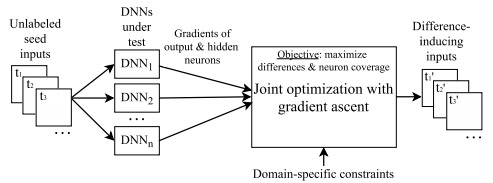
\includegraphics[width=0.8\textwidth]{xplore-wf}
    \caption{DeepXplore工作原理图\cite[图~5]{DeepXplore}}
    \label{xplore-wf}
\end{figure}

\subsection{DeepTest}[DeepTest]

DeepTest基于DeepXplore的工作,提出了一套专门针对自动驾驶系统,能够自动检测出错误行为的测试系统。发生在自动驾驶系统上的车祸大部分都是发生在一些罕见的路况场景下,而传统的自动驾驶检测测试技术几乎是完全依赖大量的罕见路况场景图片的人工收集与标注,这不仅包含了大量的人工成本,重要的是人工收集的数据无法保证能够覆盖度到了所有的极端场景数据。这些极端场景就好像是传统软件中的bug,但是这些bug一旦被检测到,就可能通过把这些导致错误的输入重新放入训练集,同时改变一下模型的结构和参数来修复。DeepTest正是通过以上的思路来设计的一套自动测试系统。

% 神经元覆盖率

具体的实现上,DeepTest依旧借用DeepXplore提出的神经元覆盖率的概念,使用位移、拉伸、仿射以及直接修改像素的透明度等基本的图形变换的手段来合成新的驾驶图像,文章里提到合成后的数据能使原DNN系统的神经元覆盖率提升100\%\cite{DeepTest},并以提升神经元覆盖率为目标,给出了一个优化算法\ref{alg1},以获得最佳的图像混合变换,最后DeepTest在利用这些合成的新数据重新训练自动驾驶模型来提高模型对于极端场景的鲁棒性。

\begin{algorithm}[h]
    \small
    \SetAlgoLined
    \SetKwInOut{Input}{Input}
    \SetKwInOut{Output}{Output}
    \SetKwInOut{Variable}{Variable}

    \Input{变换Transformations T, 种子图像Seed Images I}
    \Output{合成的测试数据图像}
    \Variable{S: 存储新合成图像的栈; Tqueue: 存储变换的队列}

    push all seed imgs to Stack S; 所有种子图片入栈\;
    $genTests = \varnothing$\;
    \While{S is not empty}{
        img = S.pop()\;
        $Tqueue = \varnothing$\;
        numFailedTries = 0 \;
        \While{$numFailedTries \leq maxFailedTries$}{
            \eIf{$Tqueue\ is\ not\ empty$}{
                T1 = Tqueue.deque()
            }{
                Randomly pick transformations T1 from T
            }
            Randomly pick parameter P1 for T1\;
            Randomly pick transformation T2 from T\;
            Randomly pick parameter P2 from T2\;
            newImage = ApplyTransforms(image, T1, P1m T2, P2)\;
            \eIf{covInc(newiamge)}{
                Tqueue.enqueue(T1)
                Tqueue.enqueue(T2)
                UpdateCoverage()
                $genTests=genTests \cup newiamge S.push(newImaghe)$
            }{
                $numFailedTries=numFailed++$
            }
        }
    }
    return genTests
    \caption{混合变换优化算法}
    \label{alg1}
\end{algorithm}

\subsection{DeepRoad}[DeepRoad]

尽管DeepTest已经提出了一个较为完善的自动驾驶系统测试方案,但它有一个很严重的缺陷,